\documentclass[../main.tex]{subfiles}

\begin{document}
	
In this project, we will focus mainly on applying the inference techniques developed in this report to the foreign exchange (\textit{forex}) market. Forex is considered to be world's largest and most liquid financial markets, and trades 24 hours a day, five days a week. It is also famous for being fast-paced and volatile, which dovetails well with high frequency trading as it provides plenty of trading opportunities and the volatility required for making significant profits. 
	
The main dataset used for testing has been obtained through the Swiss online foreign exchange bank, Dukascopy \cite{Dukascopy}. We focus mainly on the highly liquid EUR/USD currency pair, which has a high trading frequency.

We use 2 different types of foreign exchange data for testing: tick level data and fixed snapshot data. 

Tick level data is a high frequency stream-like list of transactions, with new events arriving over 100 times per second. For each transaction, we receive the transaction price together with the next closest buy (bid) and sell (ask) prices to the transaction price. An example of this data is provided in Figure \ref{fig:3__2__1__example_waveform_plots}

On the other hand, the snapshot data we obtain provides the current closest bid and ask prices at regular intervals. 

As we are most interested in high-frequency analysis of the EUR/USD data, we focus most on the tick level data. Snapshot data is used to allow us to investigate the impact of observation frequency on our trading performance. 

Next, we will examine in greater detail some key characteristics of the EUR/USD dataset that we are using to highlight any potential problems that might occur as a result of working on real exchange rates rather than simulated data. 

\subsubsection{Quantisation}

\begin{figure}[h!]
	\centering
	\subfloat[Example of EUR / USD Tick Level Data, 1600 - 1700 on 10/02/2019\label{fig:3__4__1__example_eur_usd}]{
		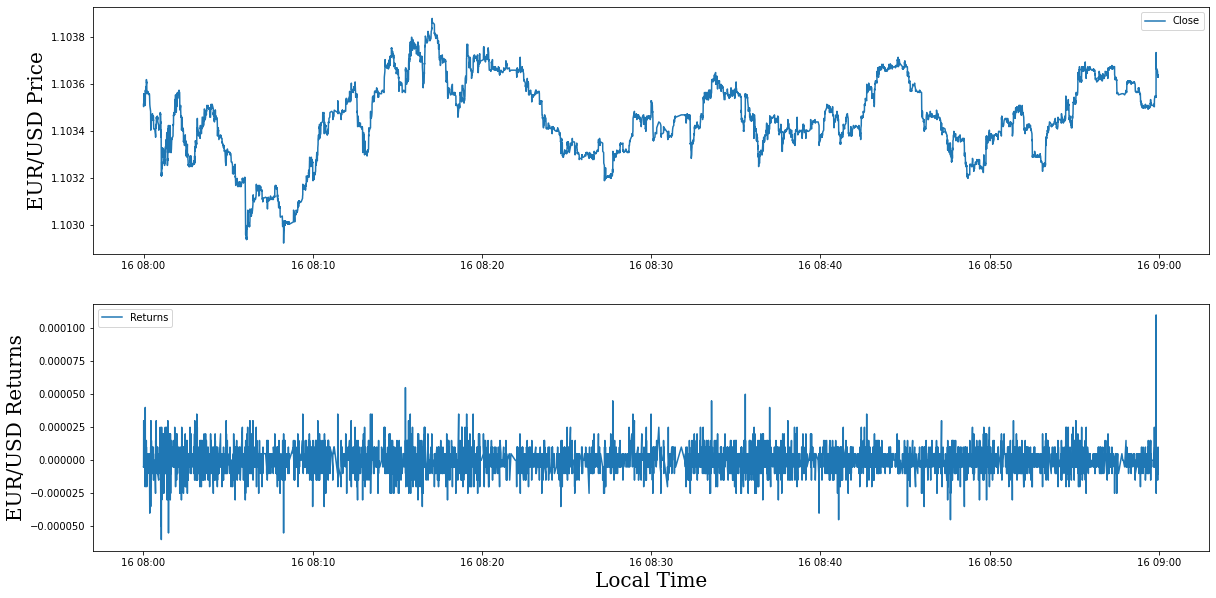
\includegraphics[width=\textwidth]{../plots/3__4__1__example_eur_usd.png}}
	\\
	\subfloat[Example of EUR / USD Daily Close Data, 1999 - 2020\label{fig:3__4__1__example_eur_usd_daily}]{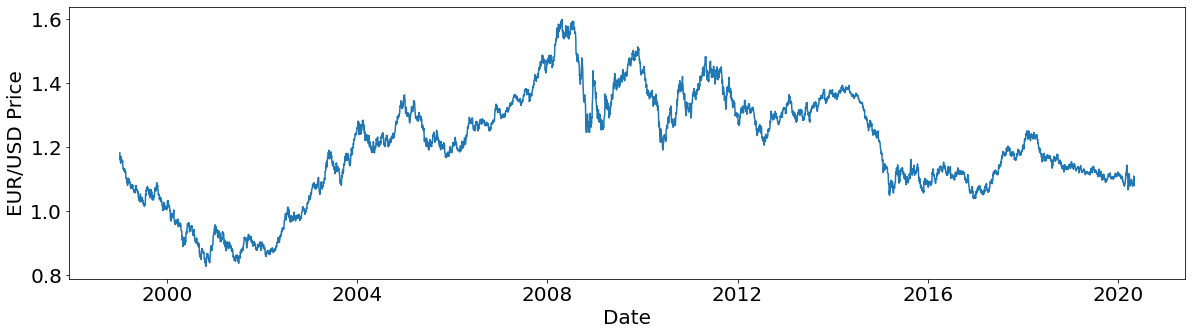
\includegraphics[width=\textwidth]{../plots/3__4__1__example_eur_usd_daily.png}}
	\label{fig:3__2__1__example_waveform_plots}
\end{figure}


The high frequency tick data that we obtain is often \textit{quantized}, and consists of only a few price levels. This is typical, as exchanges do not allow arbitrary prices to be transacted. In this case, the minimum price change possible is $5 \times 10^-6$ EUR/USD. 

This is a violation of one of the core assumptions of the stochastic modelling: that the price levels are continuous. As the minimum return ($5 \times 10^-6$) is small compared to the standard deviation of the returns, we ignore this problem in the project. However, we note that this could be a problem in extremely high frequency trading, where the price does not fluctuate much, hence causing the minimum return to be significant compared to the standard deviation of returns. 

\subsubsection{Intra-day volatility}

Unlike the stock market, the forex market is decentralised and open for trading 24 hours a day, 5 days a week. This means that there can be significant intra-day variability in the volatility of the forex data that we receive. 

Figure \ref{fig:3__2__1__intraday_vol} shows a striking example of this intra-day volatility over a 3 day period. It is readily apparent that the volatility of this particular forex exchange is high closer to European trading hours (0600 - 1800), and more muted once that time period is over. Other than this, alternative intra-day patterns have also been empirically shown to exist in many financial markets \cite{cheung1994intraday}, \cite{andersen2019time}

However, in our models we assume a constant observation noise $\sigma_{obs}$, which is directly contradicted by the presence of intra-day volatility. One way of accounting for intra-day volatility is to employ a stochastic volatility term in the state space models used to model the dynamics of the market. 

Instead of resorting to that complexity, we instead employ a simpler method. We estimate the volatility of the EUR/USD exchange rate using a GARCH(1,1) model \cite{zaffaroni2008large}, then dividing the observed returns by its estimated volatility. The intuition behind this idea is that this helps to normalise the volatility of the returns across all time periods, hence reducing the intra-day volatility observed. 

Figure \ref{fig:3__2__1__intraday_vol_repaired} shows the resultant price and volatility series obtained by applying this method, qualitatively demonstrating significant intra-day volatility reduction. 


\begin{figure}[h!]
	\centering
	\subfloat[Example of Intra-day Volatility for EUR/USD forex data\label{fig:3__2__1__intraday_vol}]{
		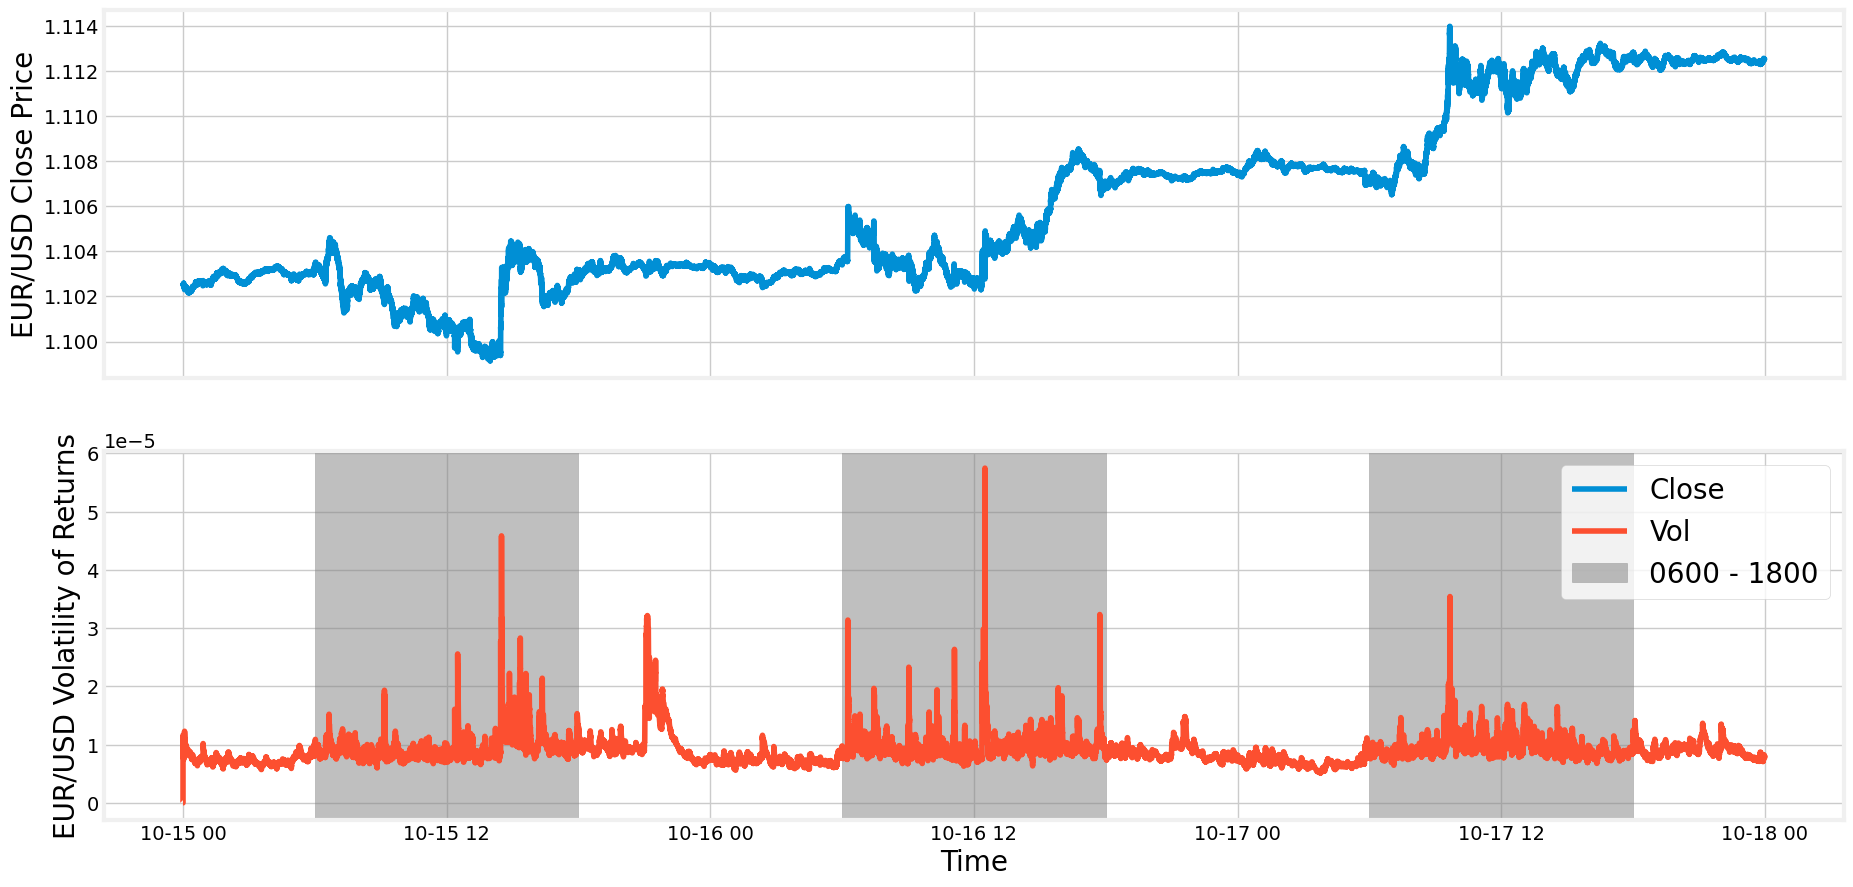
\includegraphics[width=\textwidth]{../plots/3__2__1__intraday_vol.png}}
	\\
	\subfloat[EUR/USD forex data after intra-day volatility correction\label{fig:3__2__1__intraday_vol_repaired}]{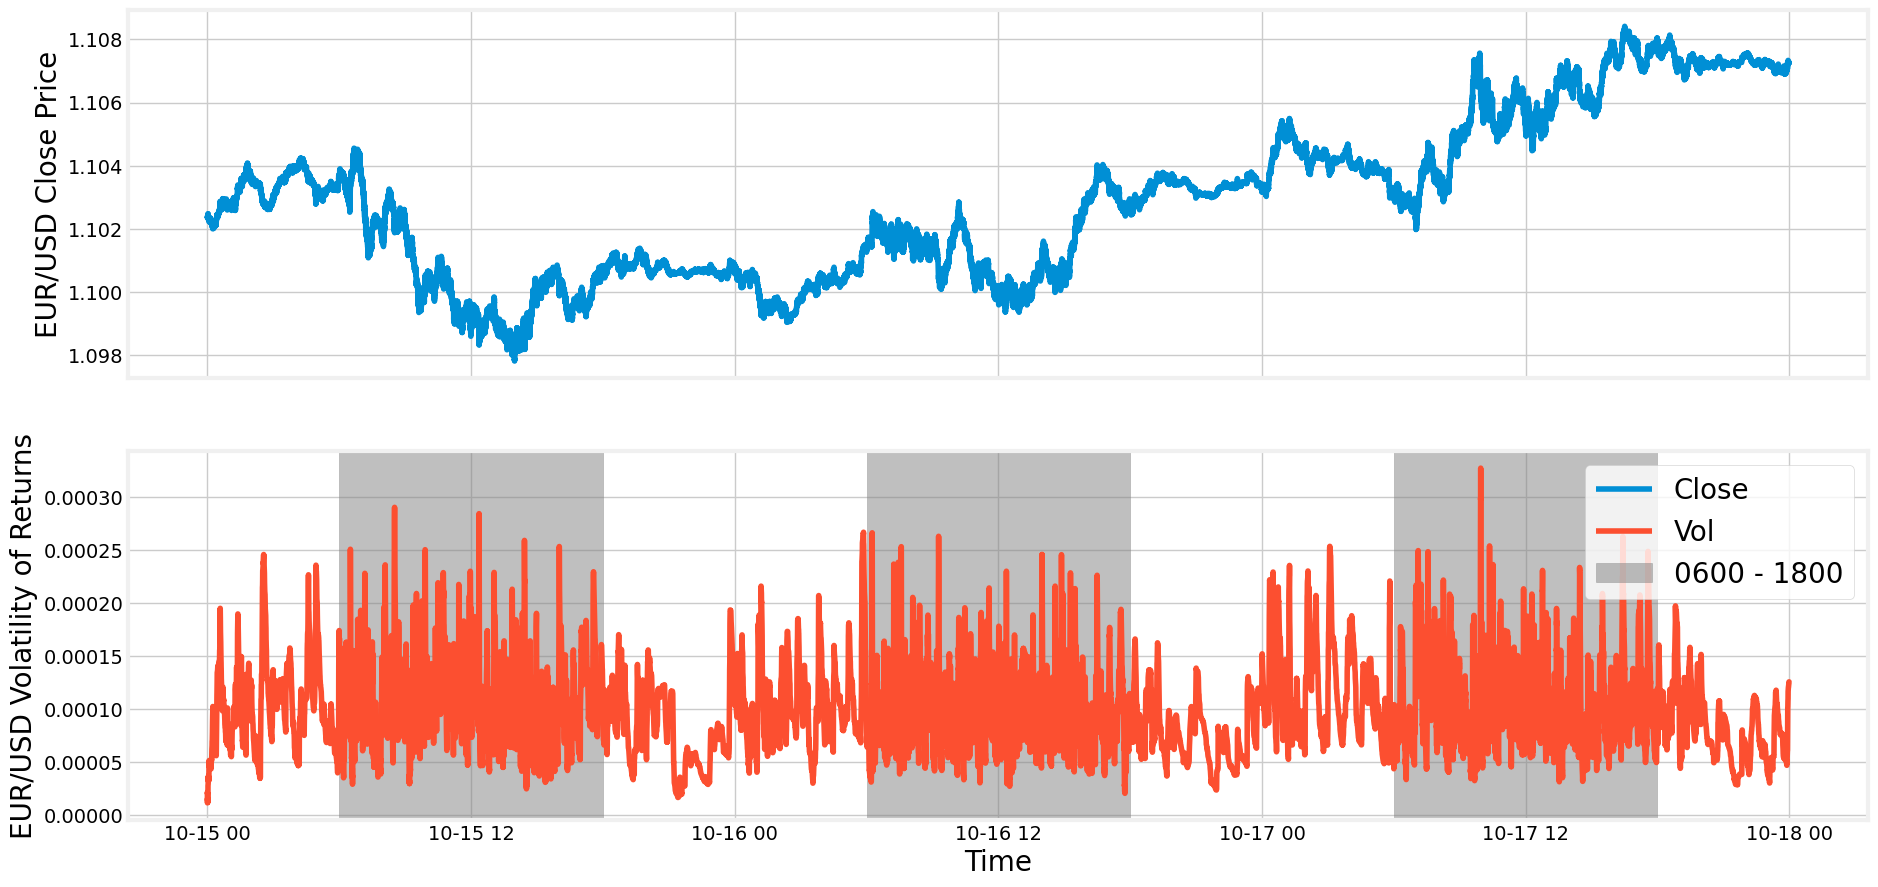
\includegraphics[width=\textwidth]{../plots/3__2__1__intraday_vol_repaired.png}}
	\label{fig:3__2__1__intraday_vol_comparison}
\end{figure}




\end{document}